\chapter{Test}\label{Test}
\setcounter{secnumdepth}{5}

\begin{longtabu} to \linewidth{@{}l l l X[j]@{}}
    Version &    Dato &    Ansvarlig &    Beskrivelse\\[-1ex]
    \midrule
\label{version_Systemark}
\end{longtabu}

\section{Indledning}
Test afsnittet giver en beskrivelse af hvilke test der løbende er blevet foretaget på både hardware og software. Testene består af modul/unit tests samt en mere omfattende integrationstest, hvor begge ligger til grund for den endelige accepttest (afsnit \ref{Accepttest}).

\section{Modul/unit test}
I dette afsnit testes enkelte delelementer af systemet uafhængigt af hinanden. Modultesten er til for at verificere de enkelte enheder virker efter hensigten.

\subsection{Hardware}
Til test af hardwaredelen blev der først udført modultest på henholdsvis forstærkeren og det analoge filter. Efterfølgende blev der udført integrationstest på forstærkeren og det analoge filter sat sammen med tryk transduceren. Slutteligt blev den samlede hardwaredel bestående af tryktransducer, forstærker og analogt filter testet på en vandsøjle.\
\subsubsection{Modul test af forstærkeren}\
I modultesten af forstærkeren blev Analog Discovery brugt som spændingsforsyning og oscilloskop på to forskellige målepunkter placeret ved henholdsvis indgangs signalet og udgangssignalet.\
Da tryktransduceren forventes at have output spændinger i området 0 til 6,25 mV blev signalet fra transduceren simuleret ved en sinus på 1 Hz med et offset på 0. Den laveste amplitude for indgangs signalet var 1 mV. For hver måling blev amplituden for indgangs signalet sat op med 1 mV indtil den sidste måling hvor amplituden var nået op på 10 mV. Således blev der 10 forskellige målinger. Reelt set var det kun nødvendigt at teste op til 6 mV eller 7 mV, da det er herimellem, at man kan forvente et max tryk fra transduceren at ligge. Da der alligevel er taget målepunkter op til 10 mV skyldes det at der ved flere målinger kan laves en ”pænere” tendenslinje ved lineær regression.

\begin{figure}[H]
	\centering
	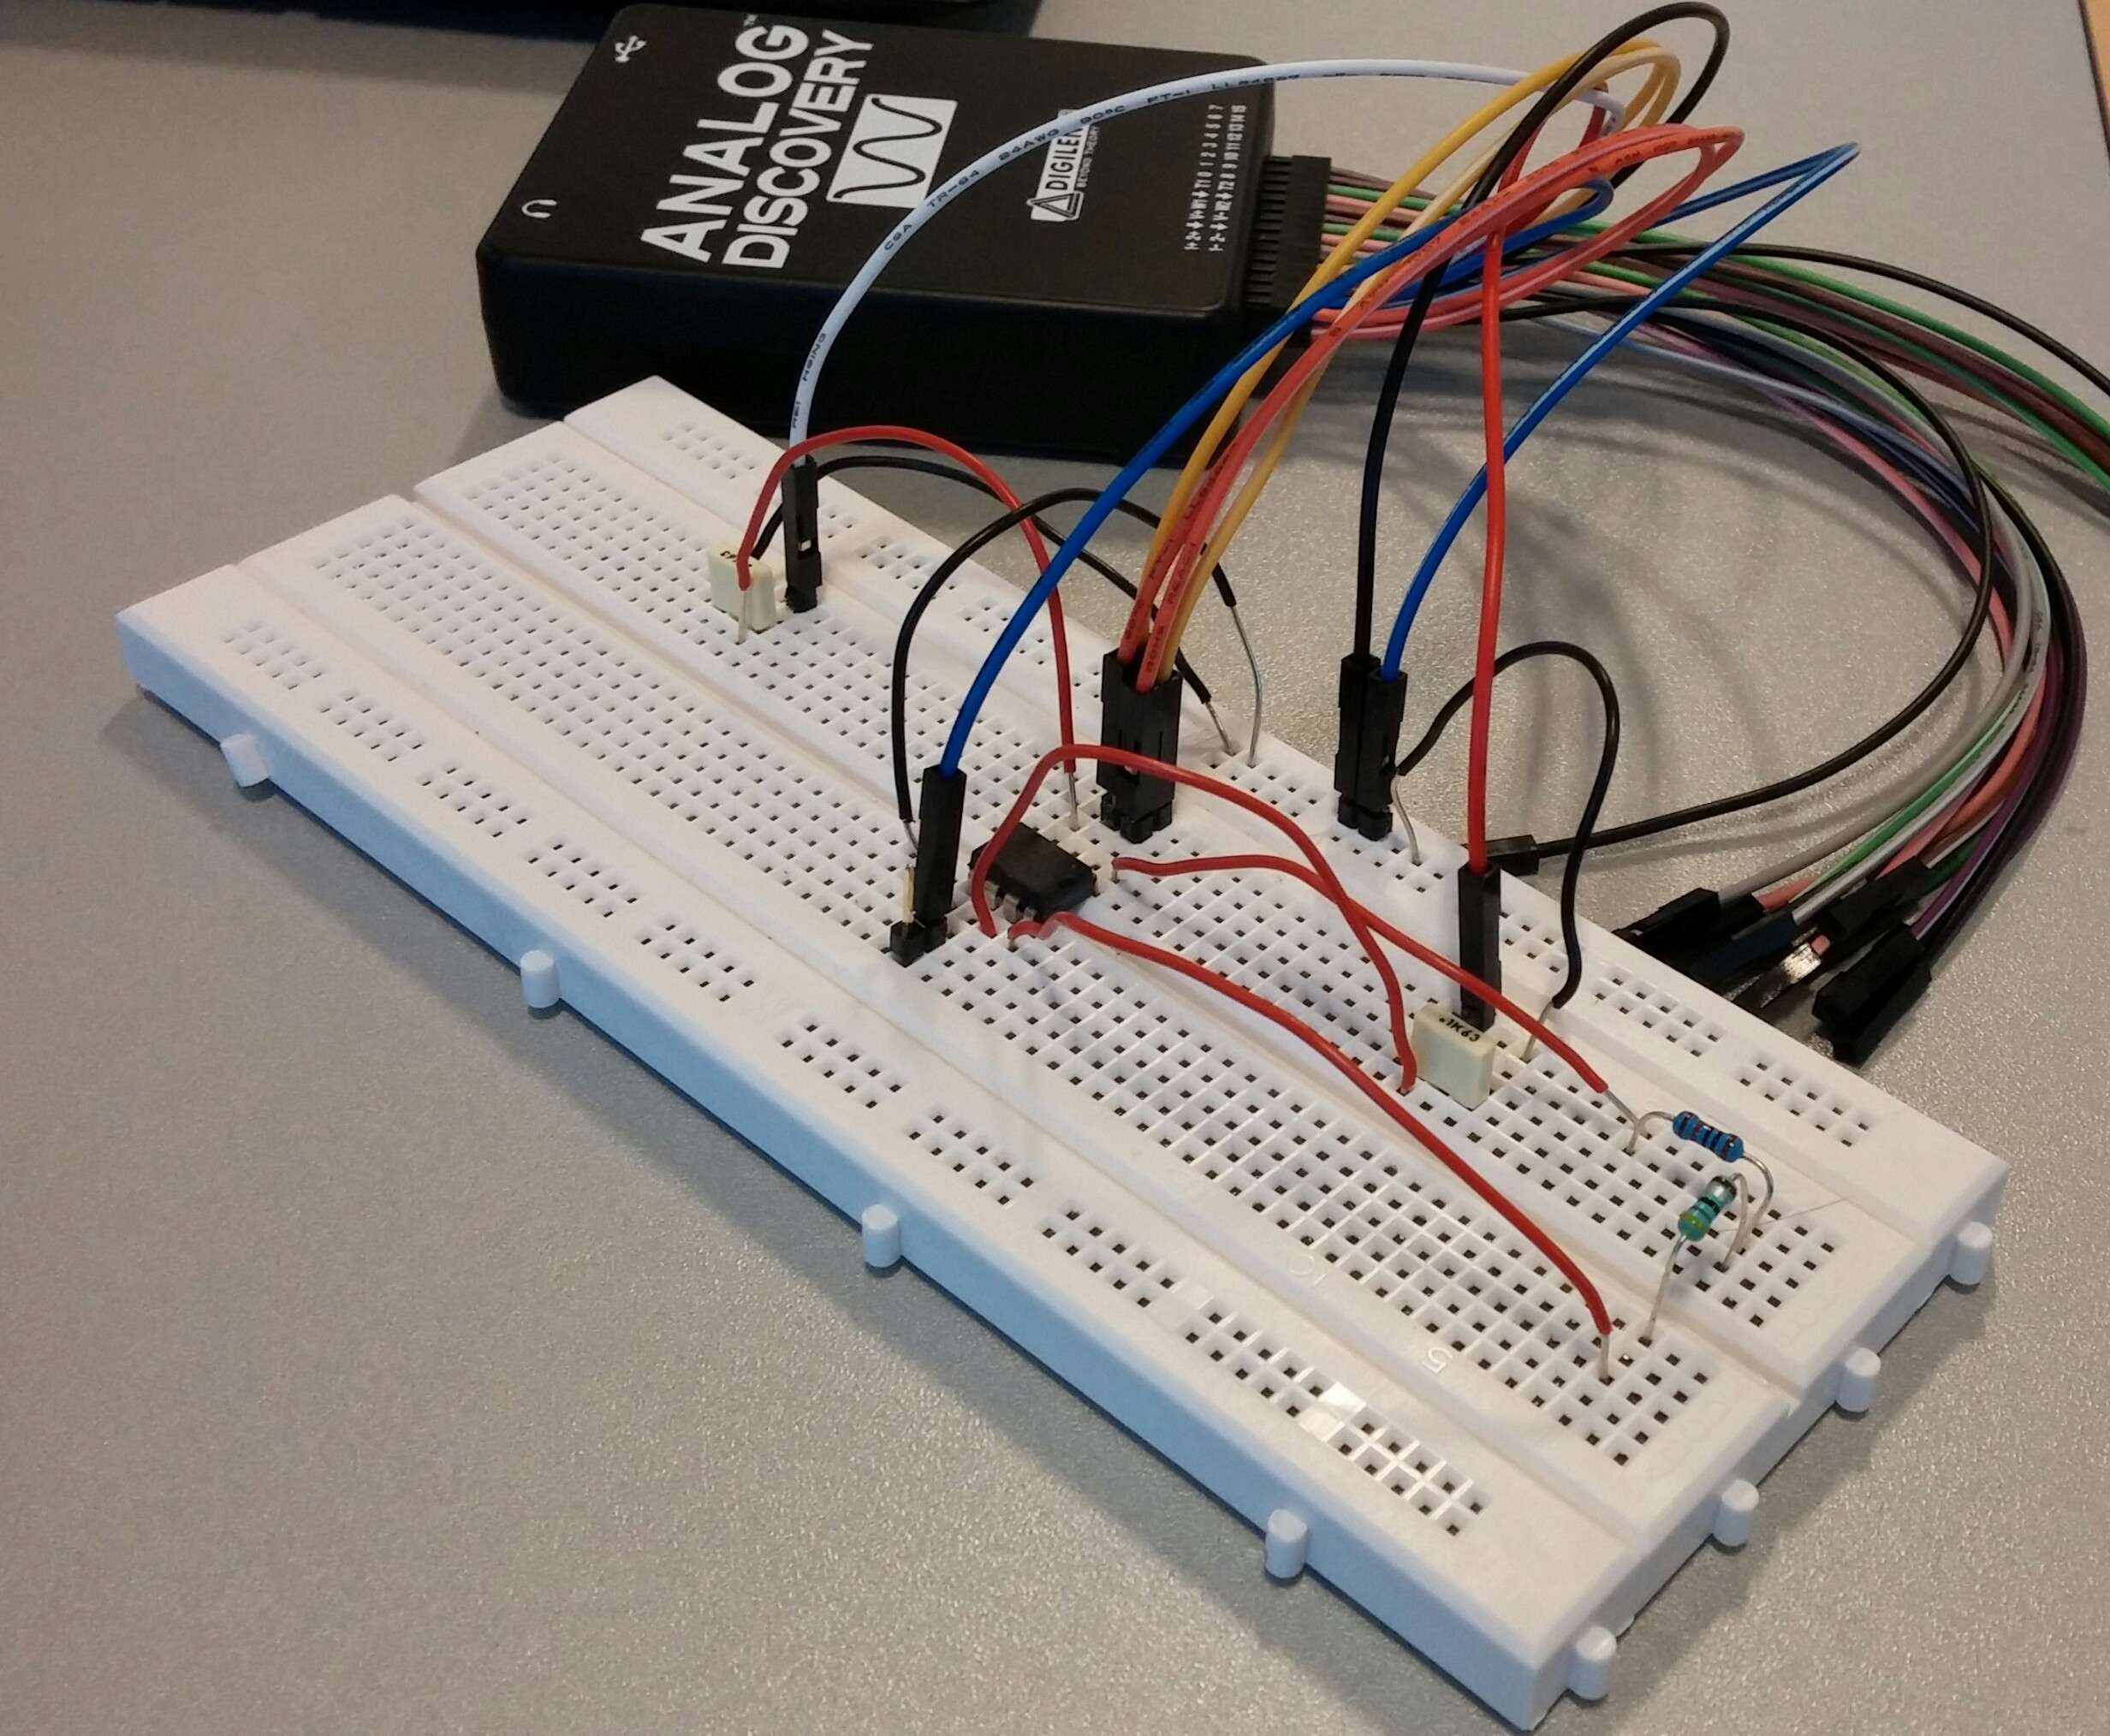
\includegraphics[width=0.5\textwidth]{Figurer/Hardware/ForstaerkerTest}
	\caption{Måleopstilling ved modul test af forstærkeren.}
	\label{fig:ForstaerkerTest}
\end{figure}

Ud af målingerne blev der foretaget lineærregression over de 10 målepunkter. Tendenslinjen der kom ud af den lineæreregression blev som følger:

\begin{center}
\begin{align}
 Y = 415,8\cdot x-0,09 \text{     hvor }R^{2} = 0,99
\end{align}
\end{center}

Her kan Y beskrives som værende forstærkningen ved en given frekvens. Konstanten 415,8 er den reelle forstærkning som er målt for forstærkeren. Skæringen med y-aksen burde være 0, men grundet måleusikkerheder er den blevet -0,09, hvilket også er acceptabelt. Den høje R$^2$ værdi indikerer, at der er en tydelig lineær sammenhænge mellem den påtrykte spænding og spændingen af output, dvs. forstærkningen er lineær.\\
Senere påtryktes samme målopstilling et DC-signal med amplituder startende fra 3mV op til 10 mV. Igen blev amplituden øget med 1 mV for hvert måling således, at der blev 7 målepunkter. Ved målinger foretaget på signaler med både 1 mV og 2 mV er offsettet i Analog Discovery så stort, at målingerne er umulige
Efter at have foretaget lineærregression på de 7 målepunkter så tendenslinjen ud som følger:

\begin{center}
\begin{align}
Y = 386,38\cdot x+0,5547\text{     hvor }R^{2} = 0,998
\end{align}
\end{center}

Forstærkningen givet ud fra de 7 måle punkter er på 386 hvilket er en del under den målte forstærkning når systemet påtrykkes et sinussignal i stedet for et DC-signal. Dette kan skyldes at der i målingen af DC-signalet er færre målepunkter, og at det dermed bliver en mere usikker måling, da selv en mindre måleusikkerhed har en større indflydelse på den målte forstærkning.

\subsubsection{Modul test af det analoge filter}
I modultesten af det analoge filter blev Analog Discovery brugt som spændingsforsyning, signal generator og som oscilloskop til at måle amplituderne for input signalet og output signalet for filteret.

\begin{figure}[H]
	\centering
	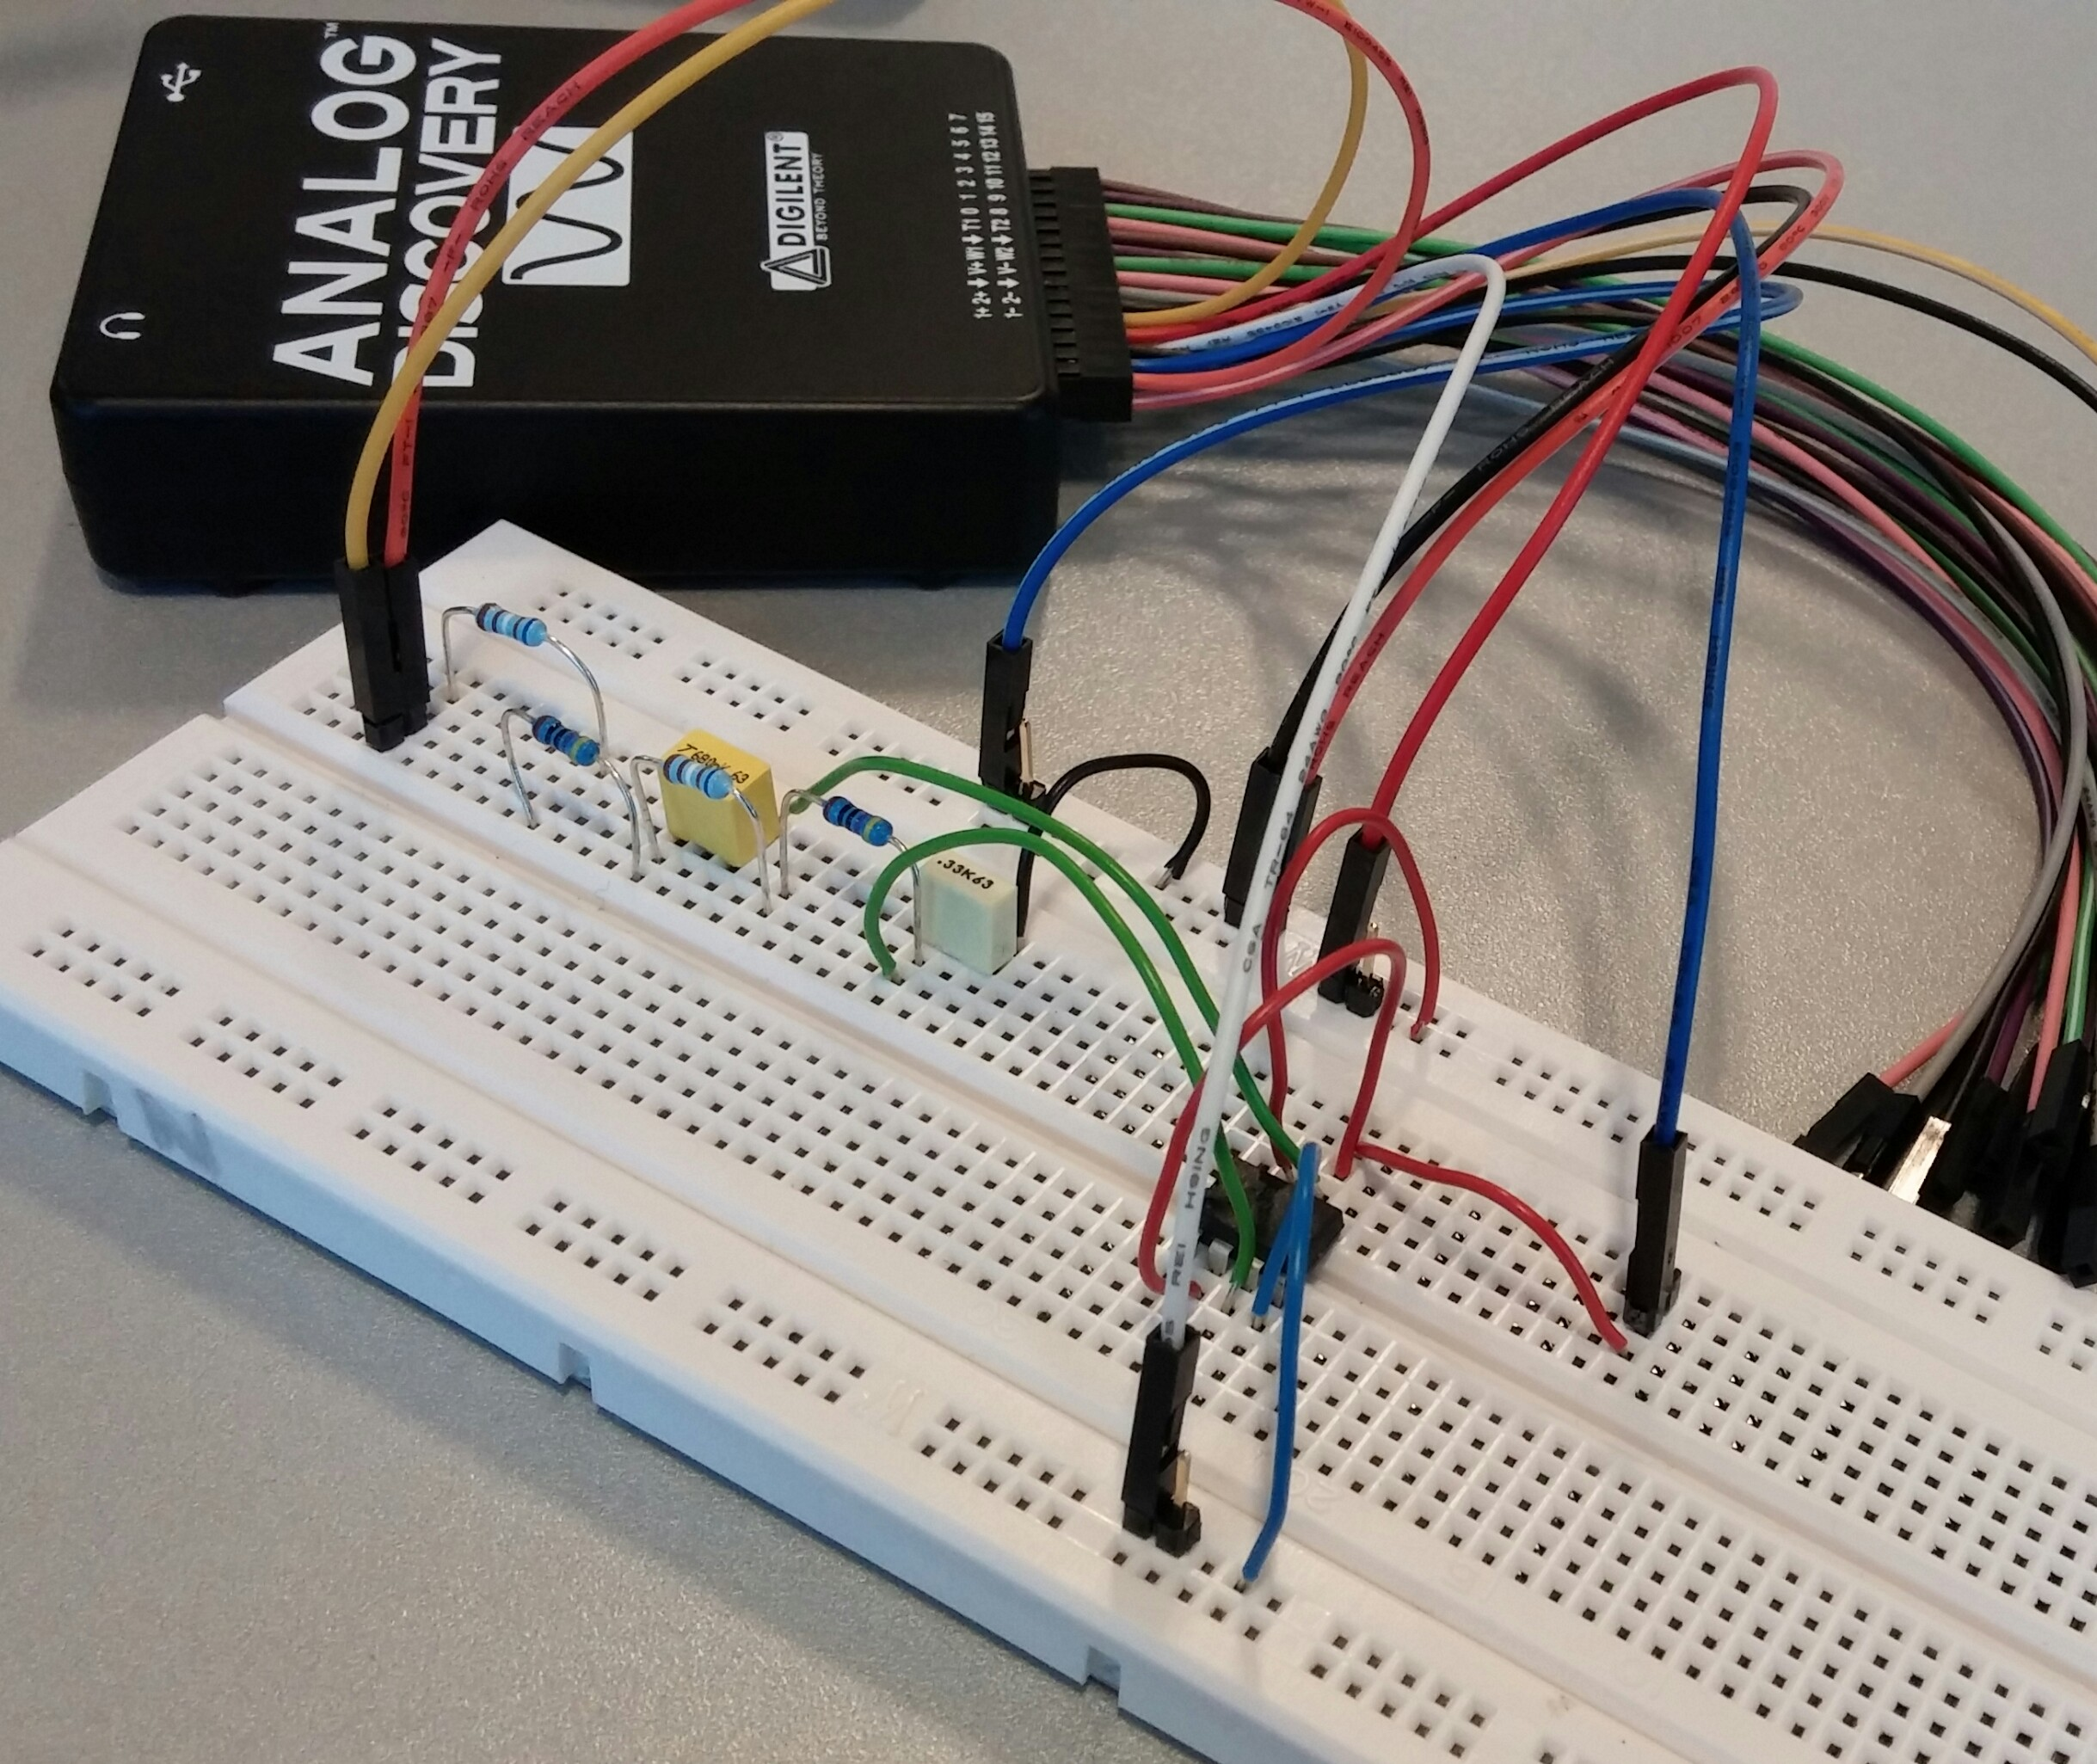
\includegraphics[width=0.5\textwidth]{Figurer/Hardware/FilterTest}
	\caption{Måleopstilling ved modultest af det analoge filter.}
	\label{fig:FilterTest}
\end{figure}

I modultesten af det analoge filter ændres frekvensen for det påtrykte sinussignal på filter indgangen. Der blev målt på i alt 21 målepunkter som lå i intervallet 1 Hz til 500 Hz, se bilag XX for de præcise angivelser af de udvalgte målefrekvenser. Output amplituden samt $\Delta$t mellem de to grafer blev aflæst på de to grafer. På baggrund af disse målinger blev dæmpningen af signalet afbildet. 

\begin{figure}[H]
	\centering
	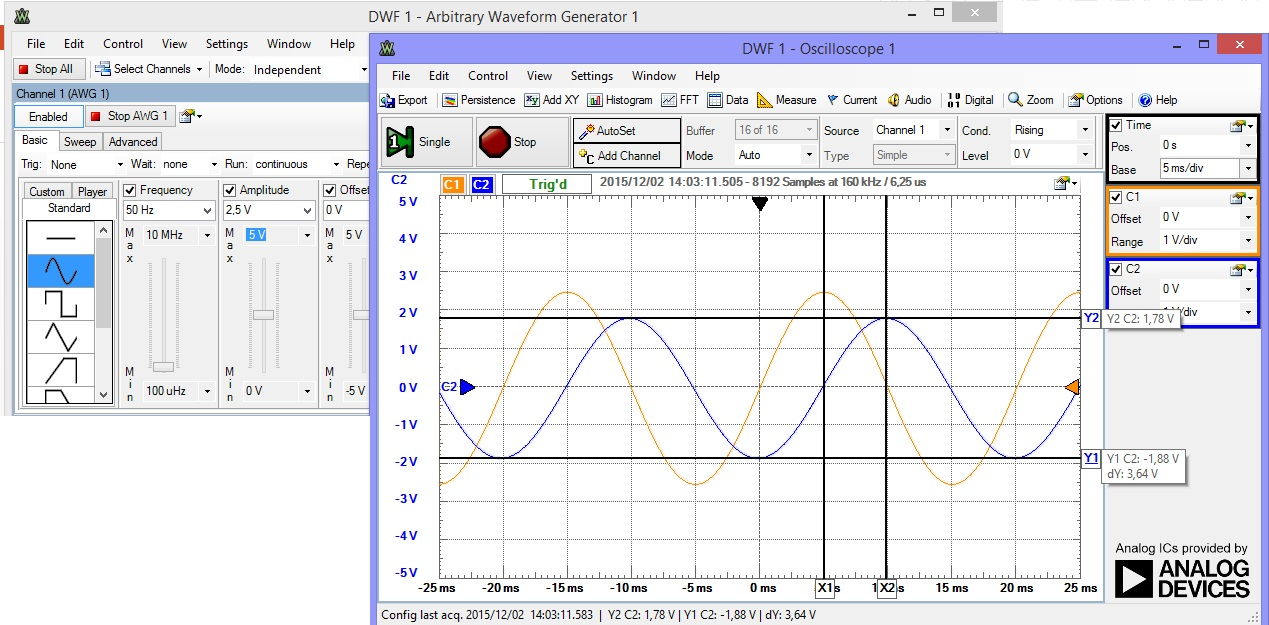
\includegraphics[width=1\textwidth]{Figurer/Hardware/AnalogScreenFilterAmp}
	\caption{Aflæsning af amplitude størrelse for outputsignalet, C2, fra filteret når inputsignalet, C1, har en amplitude på 2,5 V}
	\label{fig:FilterAmplitude}
\end{figure}

Herefter blev tidsforskydningen aflæst således at fasedrejet kunne udregnes.

\begin{figure}[H]
	\centering
	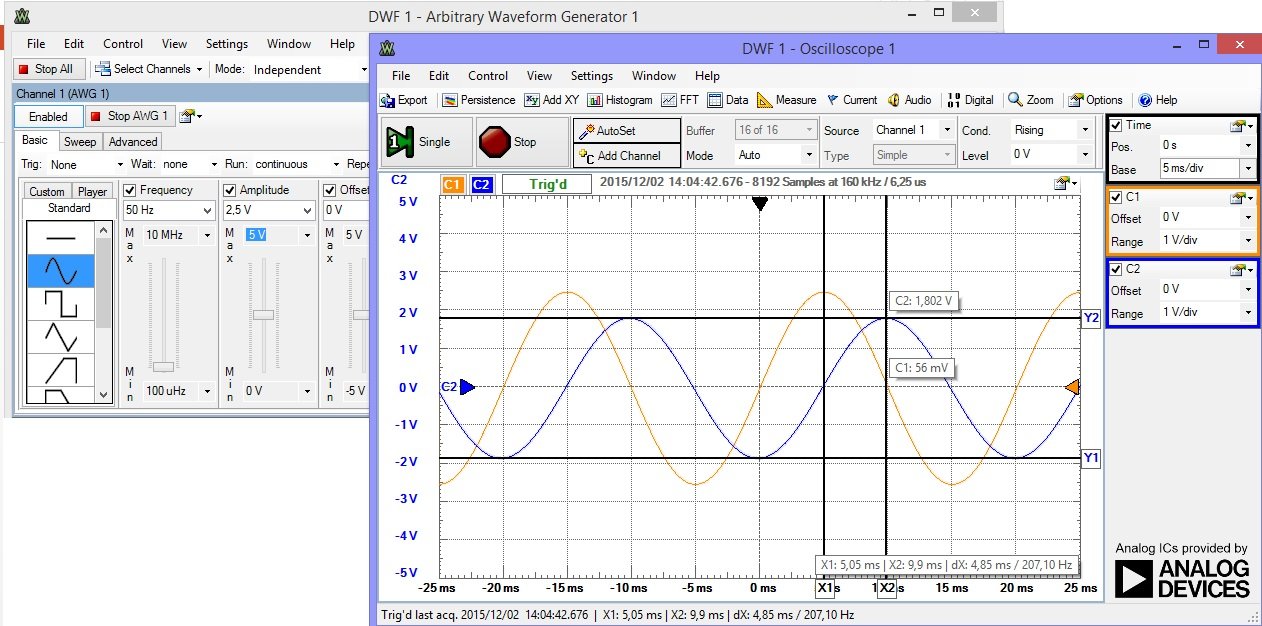
\includegraphics[width=1\textwidth]{Figurer/Hardware/AnalogScreenFilter}
	\caption{Aflæsning af tidsforskydningen for outputsignalet, C2, fra filteret set i forhold til indgangssignalet C1}
	\label{fig:FilterTidsforskydning}
\end{figure}

Det gælder generelt for et 2. ordensfilter af standarttypen som der er arbejdet med igennem projektet, at fasen er 0$^{\circ}$ en dekade før filterets knækfrekvens og falder med -90$^{\circ}$/dekade frem til dekaden efter knækfrekvensen. Derfor skal filteret i praksis have et fasedrej på minus -90$^{\circ}$ ved knækfrekvensen 50 Hz. Som det ses ud graf!! er fasedrejet ved frekvensen 5 Hz -5,2$^{\circ}$, denne skulle reelt set have været 0$^{\circ}$. 
Ved knækfrekvensen som er sat til 50 Hz er fasedrejet -86,4$^{\circ}$, hvor fasedrejet skulle have været -90$^{\circ}$. Ved målingen for 53 Hz er fasedrejet -95,4$^{\circ}$. Dermed kan der argumenteres for, at filterets reelle knækfrekvens må ligge et sted imellem 50 Hz og 53 Hz. 
For målingen på 500 Hz er fasedrejet -180$^{\circ}$, hvilket stemmer overens med teorien for 2. ordensfilterets fasekarakteristik.

\subsection{Software}
Til test af softwaren er der først og fremmest foretaget unit test af enkelte udvalgte kodelementer, for at teste om de fungerer efter hensigten. Dette er gjort ved hjælp af debug funktionen i Visual Studio.

\section{Integrationstest}

\subsection{Hardware}

\subsection{Software}
